\subsection{بخش ث}
در این بخش عبارت جبران‌ساز شتاب گرانش در دستور خروجی هدایت اضافه شده است و سپس نتایج در حضور و بدون حضور جبران‌ساز شتاب گرانش  بررسی شده است.

\begin{figure}[H]
	\centering
	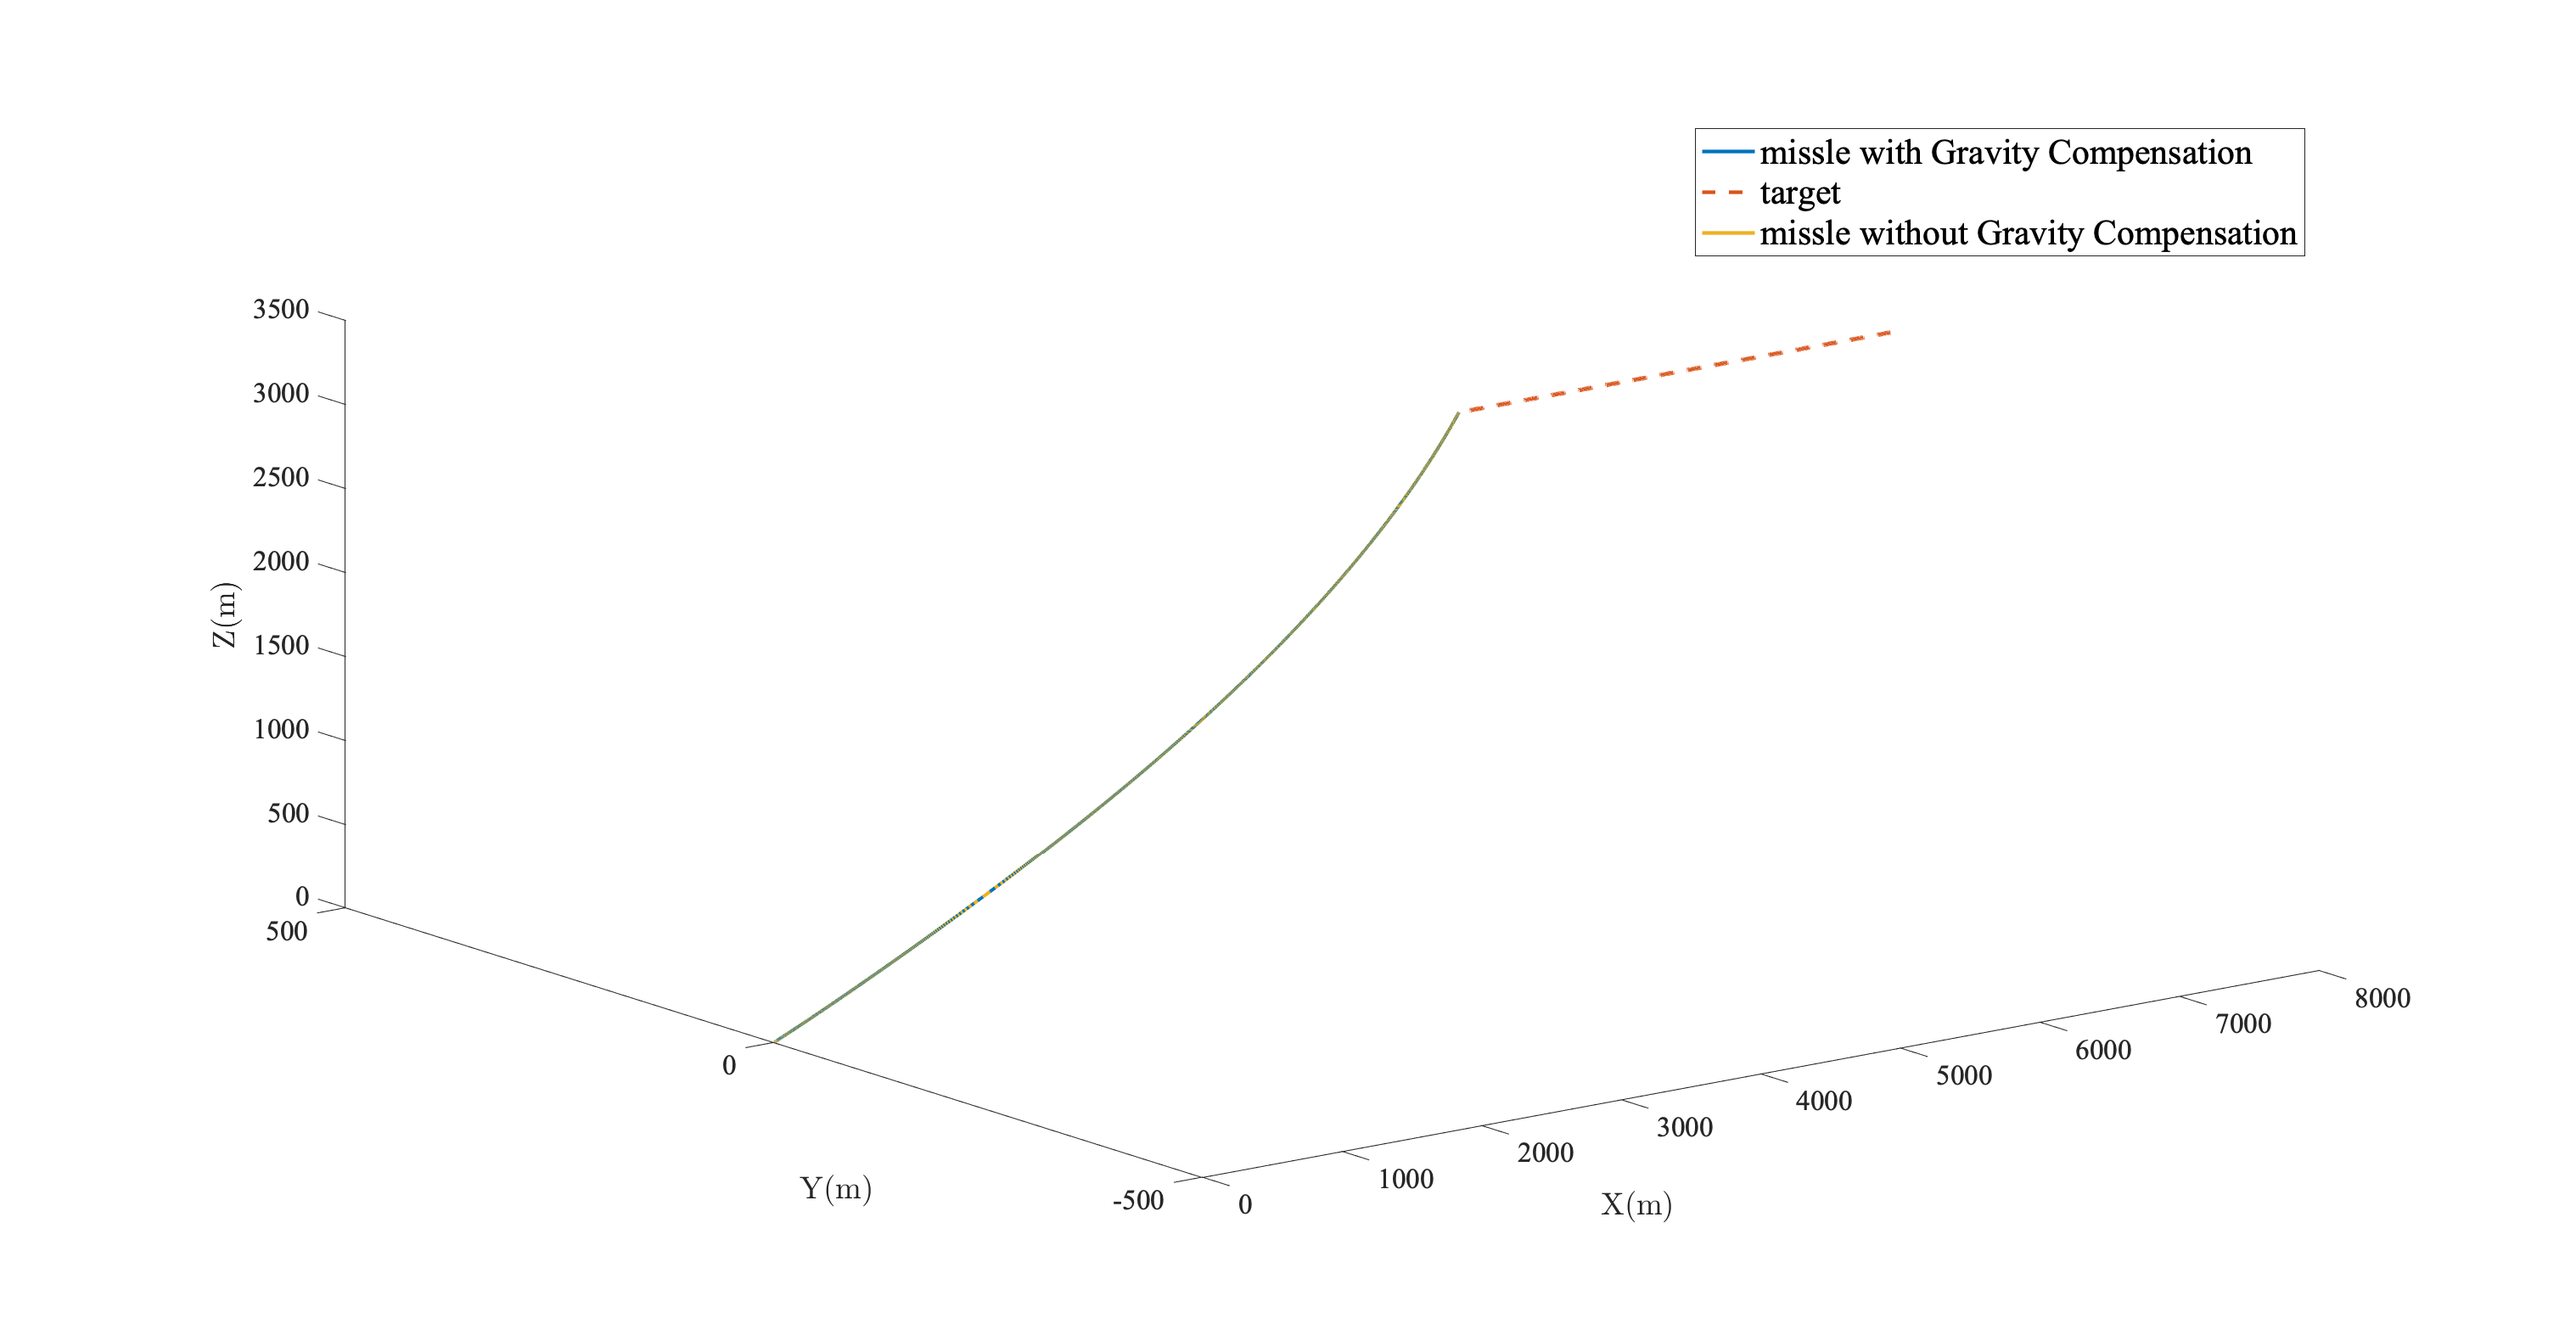
\includegraphics[width=\linewidth]{../Figure/e/3DoF_missle_vs_target_state}
	\caption{مقایسه موقعیت موشک در حضور و عدم حضور  جبران‌ساز شتاب گرانش و هدف به صورت سه بعدی  در هدایت خط دید پایه همراه با مشتق‌گیر}
\end{figure}

\begin{figure}[H]
	\centering
	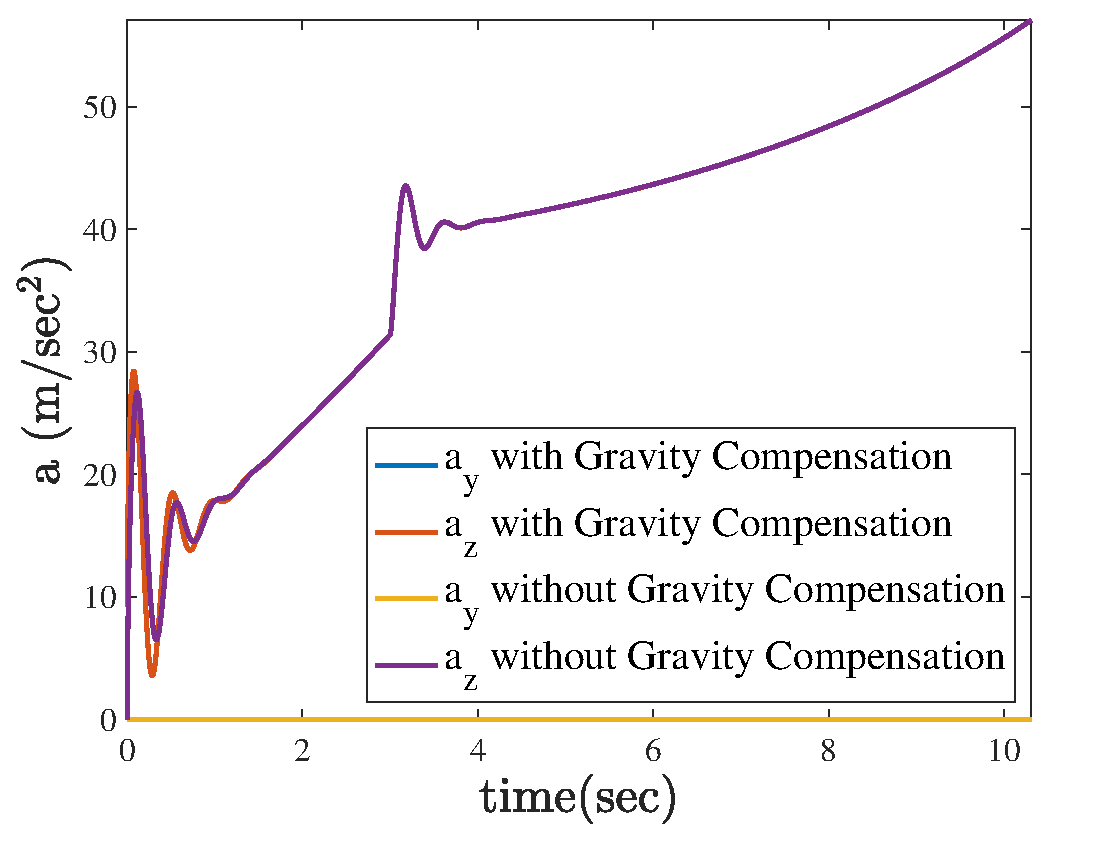
\includegraphics[width=.75\linewidth]{../Figure/e/command}
	\caption{مقایسه فرمان موشک در حضور و عدم حضور  جبران‌ساز شتاب گرانش در هدایت خط دید پایه همراه با مشتق‌گیر}
\end{figure}

\begin{figure}[H]
	\centering
	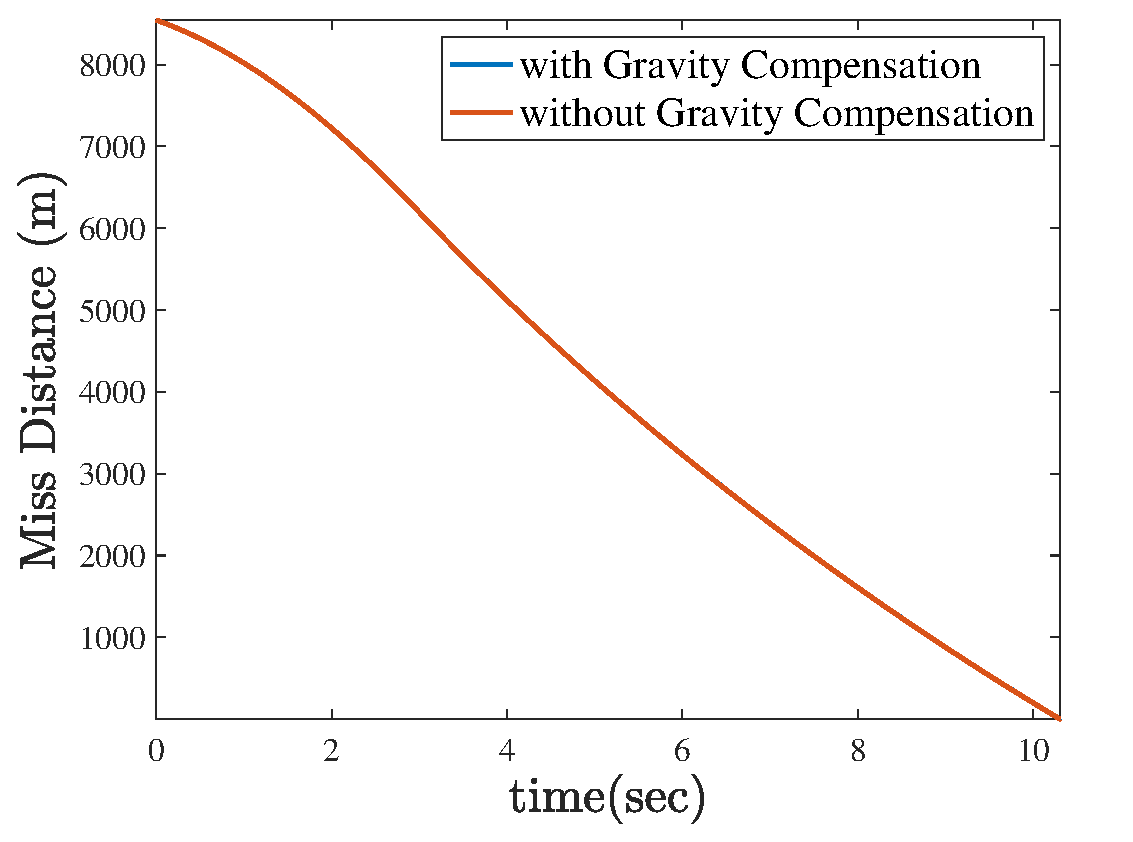
\includegraphics[width=.75\linewidth]{../Figure/e/miss_distance}
	\caption{مقایسه فاصله ازدست‌دهی موشک در حضور و عدم حضور  جبران‌ساز شتاب گرانش در هدایت خط دید پایه همراه با مشتق‌گیر}
\end{figure}

\begin{figure}[H]
	\centering
	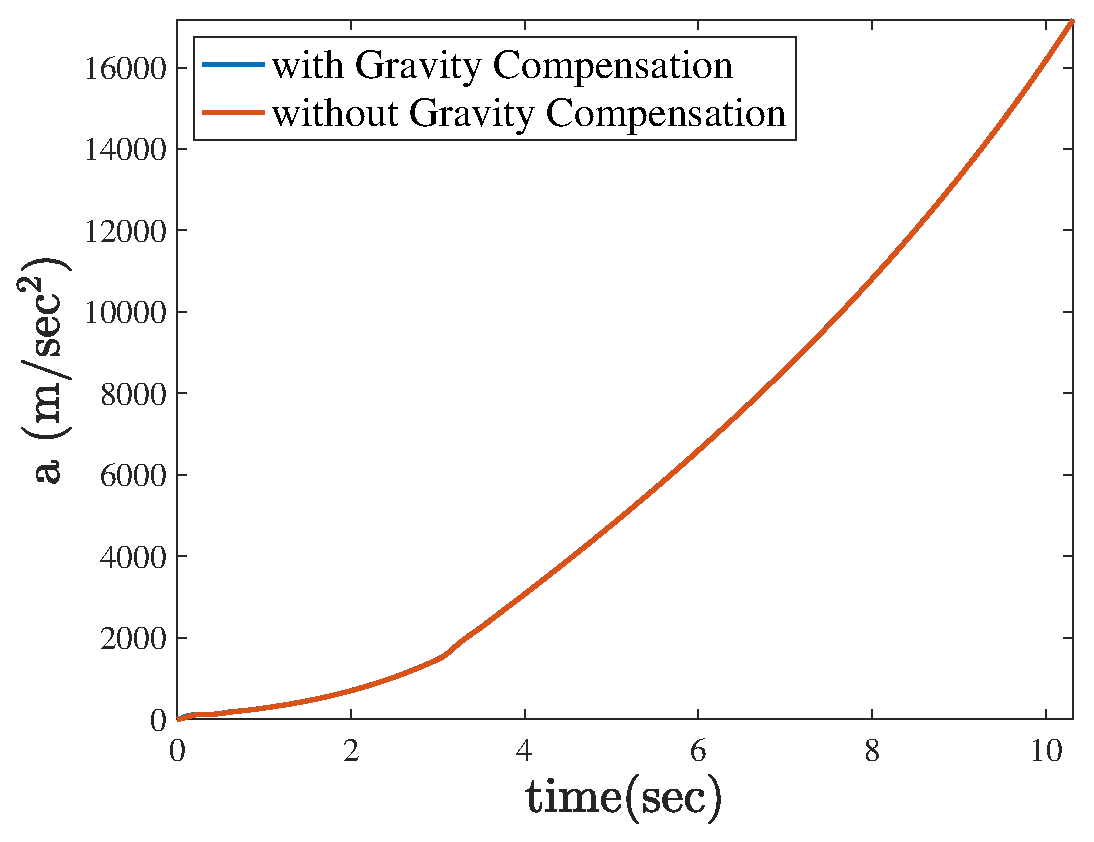
\includegraphics[width=.75\linewidth]{../Figure/e/effort}
	\caption{مقایسه مقدار تلاش کنترلی موشک در حضور و عدم حضور  جبران‌ساز شتاب گرانش در هدایت خط دید پایه همراه با مشتق‌گیر}
\end{figure}